\documentclass{article}
\usepackage[top=4cm, bottom=3cm, left=2cm, right=2cm]{geometry}
\usepackage[utf8]{inputenc}
\usepackage{amsmath}
\usepackage{nccmath}
\usepackage{amsfonts}
\usepackage[T1]{fontenc}
\usepackage{makecell}
\usepackage{graphicx}
\usepackage{caption}
\usepackage{subcaption}
\usepackage{minted}
\usepackage{pdfpages}
\usepackage[numbers]{natbib}
\usepackage[colorlinks=true, allcolors=blue]{hyperref}
\renewcommand\theadfont{\bfseries\sffamily}
\usepackage{amssymb}
\usepackage{listings}
\let\oldquote\quote
\let\endoldquote\endquote
\renewenvironment{quote}[2][]
  {\if\relax\detokenize{#1}\relax
     \def\quoteauthor{#2}%
   \else
     \def\quoteauthor{#2~---~#1}%
   \fi
   \oldquote}
  {\par\nobreak\smallskip\hfill(\quoteauthor)%
   \endoldquote\addvspace{\bigskipamount}}



\title{4M21: Software Engineering and Design}
\author{Kazal Oshodi }
\date{January 2023}

\begin{document}

\maketitle
\tableofcontents

\section{Lecture 1}
Software Engineering: a collection of methods,techniques and tools that could be applied to design, build and maintain the instructions for telling a computer what to do and how to do it
\subsection{Software Process}
\begin{itemize}
    \item Analysis: process of understanding the requirements, constraints and goals of a software development project in order to identify the best solution + alignment with stakeholder's needs
    \item Design: creating a definition of how project goals will be achieved
    \item Implementation: process of writing code - normally split into many subprojects
    \item Building: creating a complete version of software - putting all code together + custom configurations for target deployment
    \item Testing: 
    \begin{itemize} 
    \item Unit Tests: making sure that small independent parts of code work correctly 
    \item Integration Tests: all code parts work together
    \item Acceptance: functionality meets requirements
    \item Regression: New code doesn't break old
    \end{itemize}
    \item Deployment: release of software into end user environment
    \item Maintenance: supporting software during its lifetime i.e new software updates
\end{itemize}
Normally, 80-90\% of software system Total Cost Of Ownership (all costs associated with a product over its life cycle) is due to maintenance. This is because the cost of change is high + better to extend existing system to get better return on investment
\subsection{Requirement Analysis}
\begin{quote}{Fred Brooks, "No Silver Bullet - Essence and Accident in Software Engineering"}
    The hardest single part of building a software system is deciding precisely what to build
\end{quote}
It is impossible to know everything in advance required to build a system:
\begin{itemize}
    \item Users don't know 100\% what everything should do
    \item Developers don't know 100\% how users would use it
    \item Only 100\% certainty is that things will change
\end{itemize}
\subsection{Software Engineering Aims}
Software Engineering aims to manage complexity + minimise risks, as well as designing systems that can meet requirements, adapt to changes + withstand any unexpected use cases
\section{Lecture 2 - Object Oriented Programming Design and Analysis}
\subsection{Object Oriented Programming}
"Any computable function" can be achieved by:
\begin{itemize}
    \item "Sequencing" $\rightarrow$ ordered statements
    \item "Selection" $\rightarrow$ conditions, if/else
    \item "Repetition" $\rightarrow$, iterations
\end{itemize}
Object-Oriented Programming: a method of implementation in which programs are organised as cooperative collections of objects. \\ Object-Oriented Design: a method of design encompassing the process of object-oriented decomposition, i.e using objects + classes to describe the system \\
Object-Oriented Analysis: a method of analysis that examines requirements from the perspective of the classes and objectives found in the vocabulary of the problem domain
\subsection{Abstraction}
We can use an object-oriented approach to describe a system in terms of meaningful abstractions (classes), relationship and interactions between them. \\ Abstractions are generalisations that define certain key characteristics and behaviours e.g all cars have 4 wheels. \\ In Object-oriented design, recognising the sameness amongst things can allow us to create abstractions which cause smaller applications and simpler architectures. \\ Abstraction is about: 
\begin{itemize}
    \item Dealing with ideas
    \item Generalisation 
    \begin{itemize}
        \item To focus on what matters - on key characteristics and behaviours
        \item To simplify and make complexity more manageable
    \end{itemize}
\end{itemize}
\subsubsection{Class}
A class encapsulates data and behaviour. When thinking about object-oriented design, need to consider:
\begin{itemize}
    \item What classes of objects are present in the problem?
    \item What behaviour should each class provide?
    \item What should happen when an action is requested of an object?
\end{itemize}
\begin{figure}[H]
\centering
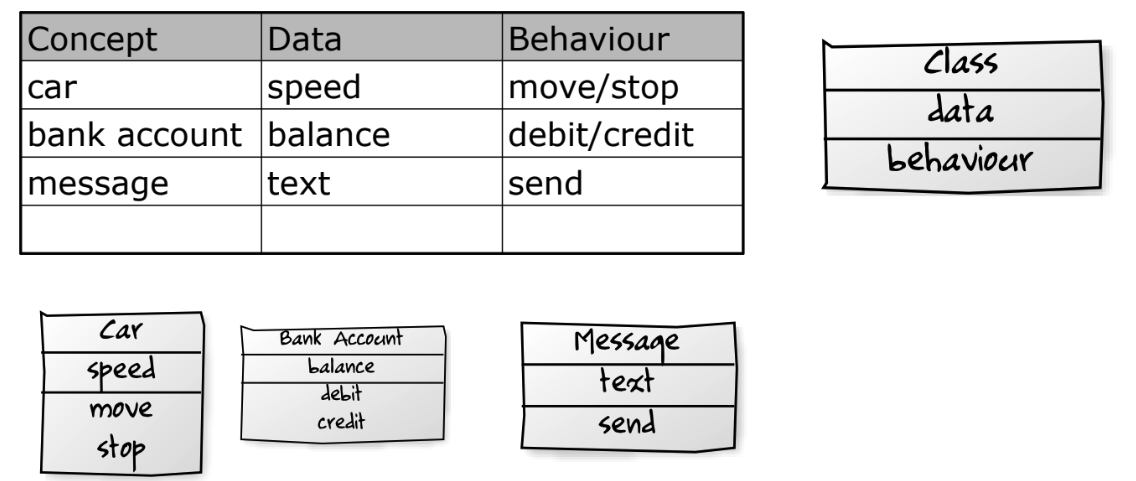
\includegraphics[width = 0.5\linewidth]{Pictures/Screenshot 2023-01-25 at 11.43.59.png}
\caption{Example of classes}
\end{figure}
Note however, that we don't want an abundance of classes. Each class might only be useful for a particular application, and thus should be used for that purpose. For example, a student in the view of the Teaching Office is characterised by the modules they are taking, whereas from the tutor viewpoint they are characterised by their wellbeing.
\subsubsection{Object}
Each class can create multiple instances (objects), which can contain data/behave like the class it is made from. For example the bank account class can be used to create two bank accounts which can credit/debit cash
\begin{figure}[H]
\centering
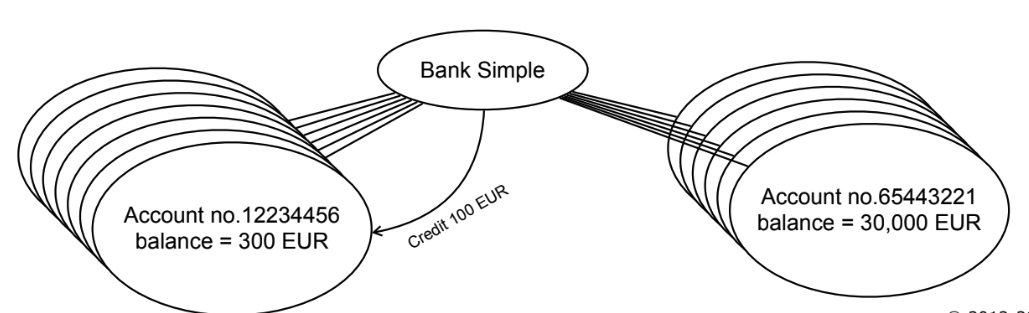
\includegraphics[width = 0.5\linewidth]{Pictures/Screenshot 2023-01-25 at 11.46.39.png}
\caption{Two Objects derived from the same class}
\end{figure}
\subsubsection{Encapsulation}
Classes can provide abstraction. This means that an object can be used without the knowledge of how it works. We want to expose only what it can do and not how, e.g that a steering wheel will make a car turn left if we turn it left, without any knowledge about how this occurs. This is encapsulation \\ \\ Suppose a person has a Name attribute. If we want to access the Name, we could do this directly:
\begin{minted}{Java}
class Person 
{
    public String FIRST_NAME = "John"
    public String LAST_NAME = "Smith"
}
print Person.FIRST_NAME + Person.LAST_NAME
\end{minted}
But, if we wanted to print the last name first e.g in France, then we could:
\begin{minted}{Java}
if (in France)
    print Person.LAST_NAME + Person.FIRST_NAME
else
    print Person.FIRST_NAME + Person.LAST_NAME

\end{minted}
But, it would be easier to keep Name variables hidden (encapsulation), and just use a method to access them instead:
\begin{minted}{Java}
class Person
{
    private String FIRST_NAME = "John"
    private String LAST_NAME = "Smith"

    public String NAME
    {
    if (in France)
        return Person.LAST_NAME + Person.FIRST_NAME
    else 
        return Person.FIRST_NAME + Person.LAST_NAME
    }
}
print Person.NAME
\end{minted}
We use encapsulation to:
\begin{itemize}
    \item Hide implementation
    \item Reduce dependencies between different parts of the application - decoupling
    \item Make changes safely
    \item Debug easier
    \item Make everything more manageable
\end{itemize}
Thus we should try to encapsulate as much as possible.
\subsubsection{Getters/Setters}
We use getters and setters to allow for controlled access to internal data fields.
\begin{minted}{Java}
class Person
{
    private String email;
    public String getEmail {
        return email;
    }
    public setEmail( String newEmail) {
    if ((newEmail != null) && (newEmail.contains('@'))){
        email = newEmail;
    }
    }
}
\end{minted}
We can do this to implement constraint checking, as well as control concurrent access - allowing only one thread to access an object at a time. It also allows for the actual data source to be hidden so it can't be access. \\ \begin{quote}{Martin Fowler}
    The point of encapsulation isn't really about hiding the data, but hiding design decisions, particularly in areas where those decisions may have to change. 
\end{quote}
For example, if you want to communicate with an external data source, use encapsulation, because we want to focus on the messages delivered to the data source rather than the data source itself. \\ If we don't have controlled access to internal data fields, then this means that:
\begin{itemize}
    \item We can't abstract the class
    \item We can't remove/reduce dependencies between different parts of the system
    \item We can't make changes safely
    \item We can't debug quickly
\end{itemize}
Thus, we should hide everything except what we want to expose.
\subsection{Inheritance}
Classes can be related: 
\begin{itemize}
    \item Superclass/base class (parent) can be extended/inherited from
    \item Subclass (child) extends/inherits from superclass
\end{itemize}
Each subclass can do everything a superclass can, but they can also:
\begin{itemize}
    \item Hold additional data
    \item Perform new actions
    \item Perform original actions differently
\end{itemize}
For example with a shape:
\begin{figure}[H]
\centering
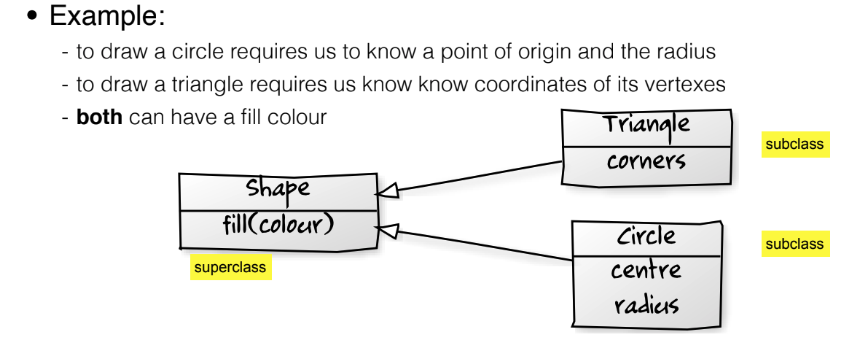
\includegraphics[width = 0.5\linewidth]{Pictures/Screenshot 2023-01-25 at 13.26.24.png}
\caption{Inheritance}
\end{figure}
\subsection{Polymorphism}
Polymorphism allows us to request the same action from objects, but execute it in different ways. For example, if we have different bank accounts, but we want to find out how much money is in each account, then the action is the same - request the current balance. However, the way the balance could be calculated could be different. But we can still use polymorphism to simplify our code. This is an example of class inheritance hierarchy, which lets us choose the level of abstraction at which we interact with an object. \\ For example, compare this code:
\begin{minted}{Java}
for CurrentAccount in Bank 
{
    TotalMoney += CurrentAccount.balance()
}
for SavingAccount in Bank 
{
    TotalMoney += SavingAccount.balance()
}
for SuperHighInterestAccount in Bank 
{
    TotalMoney += SuperHighInterestAccount.balance()
}
\end{minted}
To this code:
\begin{minted}{Java}
for Account in Bank
{
    TotalMoney += Account.balance()
}
\end{minted}
\begin{figure}[H]
\centering
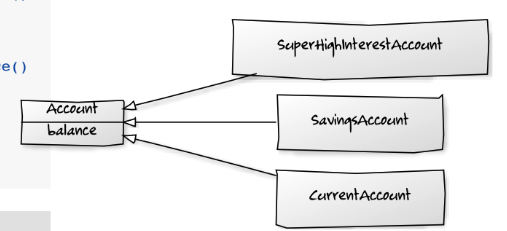
\includegraphics[width = 0.5\linewidth]{Pictures/Screenshot 2023-01-25 at 13.33.03.png}
\caption{Polymorphism}
\end{figure}
Polymorphism seperates the declaration of functionality from the specifics of its implementation.
\subsection{Identifying good Classes}
Remember: Inheritance "IS A" Relationship - Subclass "IS A" Superclass i.e Coffee IS A Drink, Car IS A Vehicle
\begin{figure}[H]
\centering
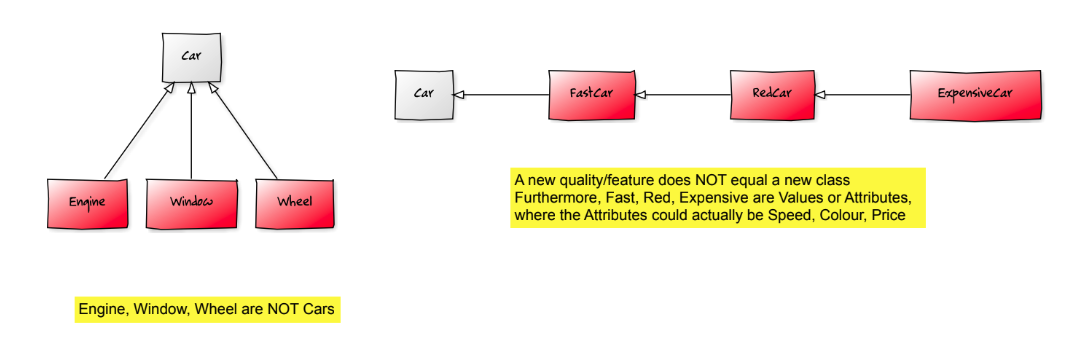
\includegraphics[width = 0.8\linewidth]{Pictures/Screenshot 2023-01-25 at 13.36.04.png}
\caption{Bad Classes}
\end{figure}
\subsection{Abstract Classes}
We want our classes to be abstract - a class which can't be instantiated. This means that we can't define the class without going into more detail. This is good for capturing the higher level view of a system
\begin{figure}[H]
\centering
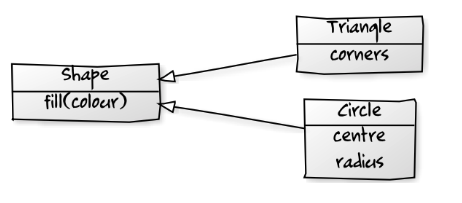
\includegraphics[width = 0.5\linewidth]{Pictures/Screenshot 2023-01-25 at 13.37.34.png}
\caption{Abstract Class}
\end{figure}
\subsection{Interfaces}\label{interface}
An interface is a purely abstract class which defines only behaviour - not data. This is a point where two entities meet and interact. It defines a set of ways to interact with a class, or a contract of what must be avaliable. Interfaces help to add specific behaviour to classes. Most classes with extend one superclass, but will implement multiple interfaces.
\begin{figure}[H]
\centering
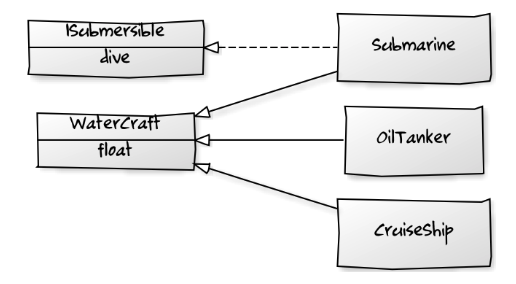
\includegraphics[width = 0.5\linewidth]{Pictures/Screenshot 2023-01-25 at 13.39.41.png}
\caption{Interfaces}
\end{figure}
\pagebreak
\section{Lecture 3 -Introduction to UML}
UML is a formal graphical language which has a set of diagrams for describing software systems. This can be used for designing, documenting and communicating software architecture + program behaviour. \\
There are 14 types of diagrams defined:
\begin{figure}[H]
\centering
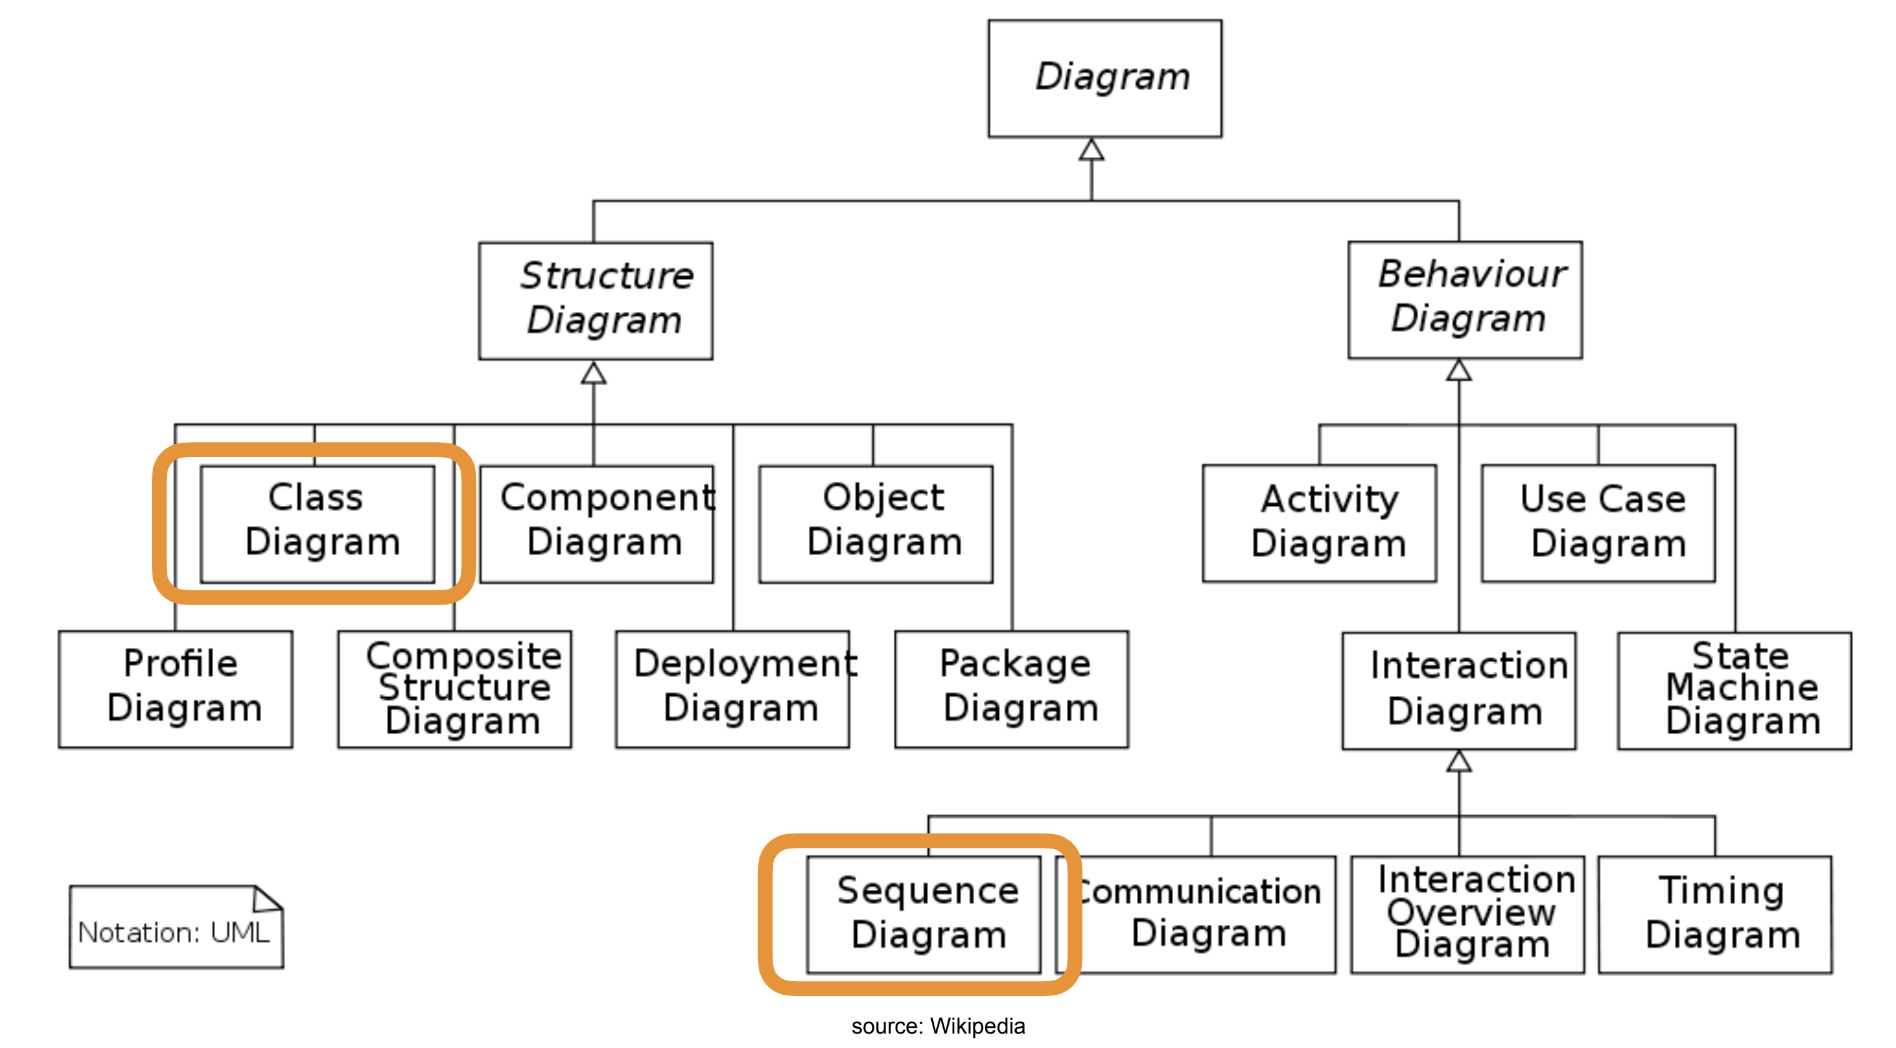
\includegraphics[width = 0.5\linewidth]{Pictures/Screenshot 2023-01-27 at 12.04.06.png}
\caption{UML Types}
\end{figure}
To describe a system we need:
\begin{itemize}
    \item Structures: Items + how they are connected
    \item Behaviour: How items interact
\end{itemize}
UML, we use Class Diagrams to represent structures. These describe the software architecture by explaining what classes are in a system + their relationships. \\
Behaviour diagrams such as Sequence and Communication Diagrams show interaction between objects. \\
We want to use UMLAsSketch to communicate parts of the system to a group of people.
\subsection{Class Diagram}
These show the classes in a software system, along with their attributes, operations and relationships:
\begin{figure}[H]
\centering
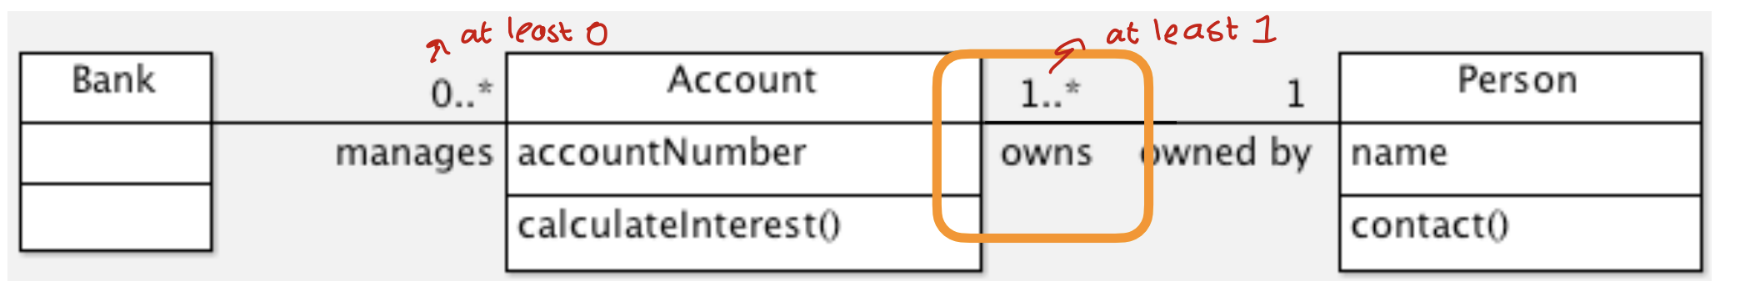
\includegraphics[width = 0.8\linewidth]{Pictures/Screenshot 2023-01-27 at 12.09.45.png}
\end{figure}
Explaining this diagram: 
\begin{itemize}
    \item Bank can manage at least 0 accounts
    \item An Account has an account number and can calculate interest
    \item Each Account can be owned by one Person
    \item One Person can own multiple accounts
    \item Each Person has a name and can be contacted
\end{itemize}
Each class is represented by 3 different sections: name, attributes and operations/methods:
\begin{figure}[H]
\centering
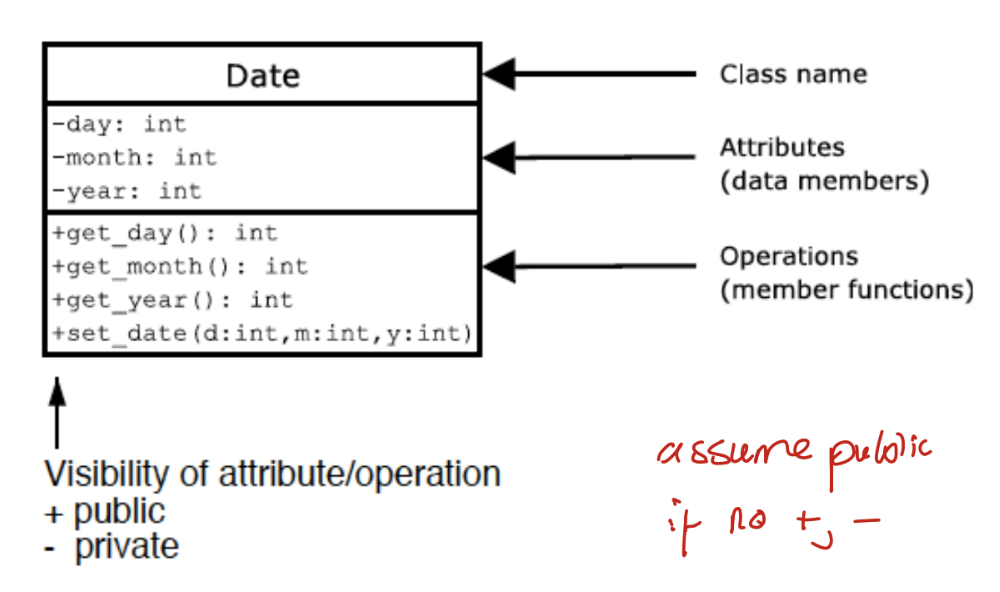
\includegraphics[width = 0.6\linewidth]{Pictures/Screenshot 2023-01-27 at 12.12.02.png}
\end{figure}
We try to only include public features of a class in UML as they can be used in relation with other classes.
\begin{figure}[H]
\centering
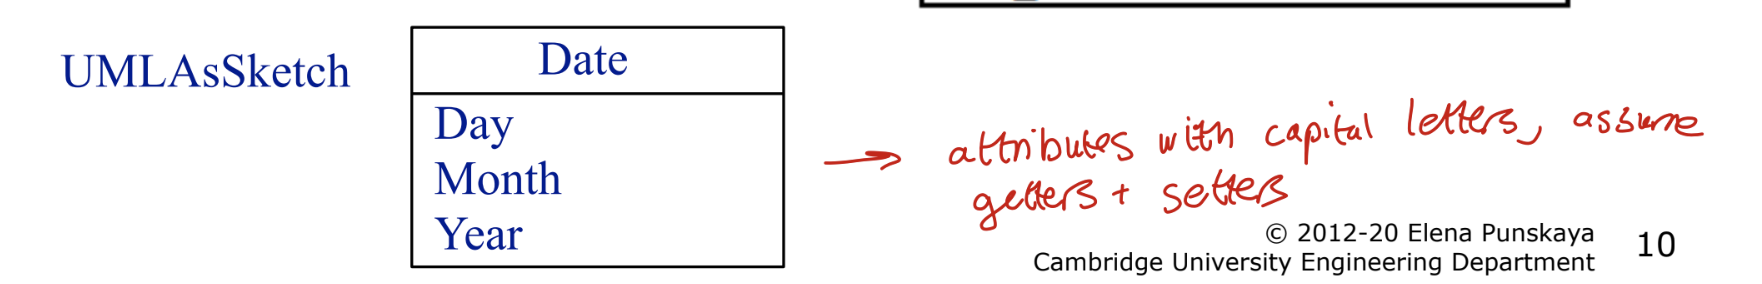
\includegraphics[width = 0.6\linewidth]{Pictures/Screenshot 2023-01-27 at 12.13.24.png}
\end{figure}
We want to have the right level of abstraction to keep the diagrams concise and useful:
\begin{figure}[H]
\centering
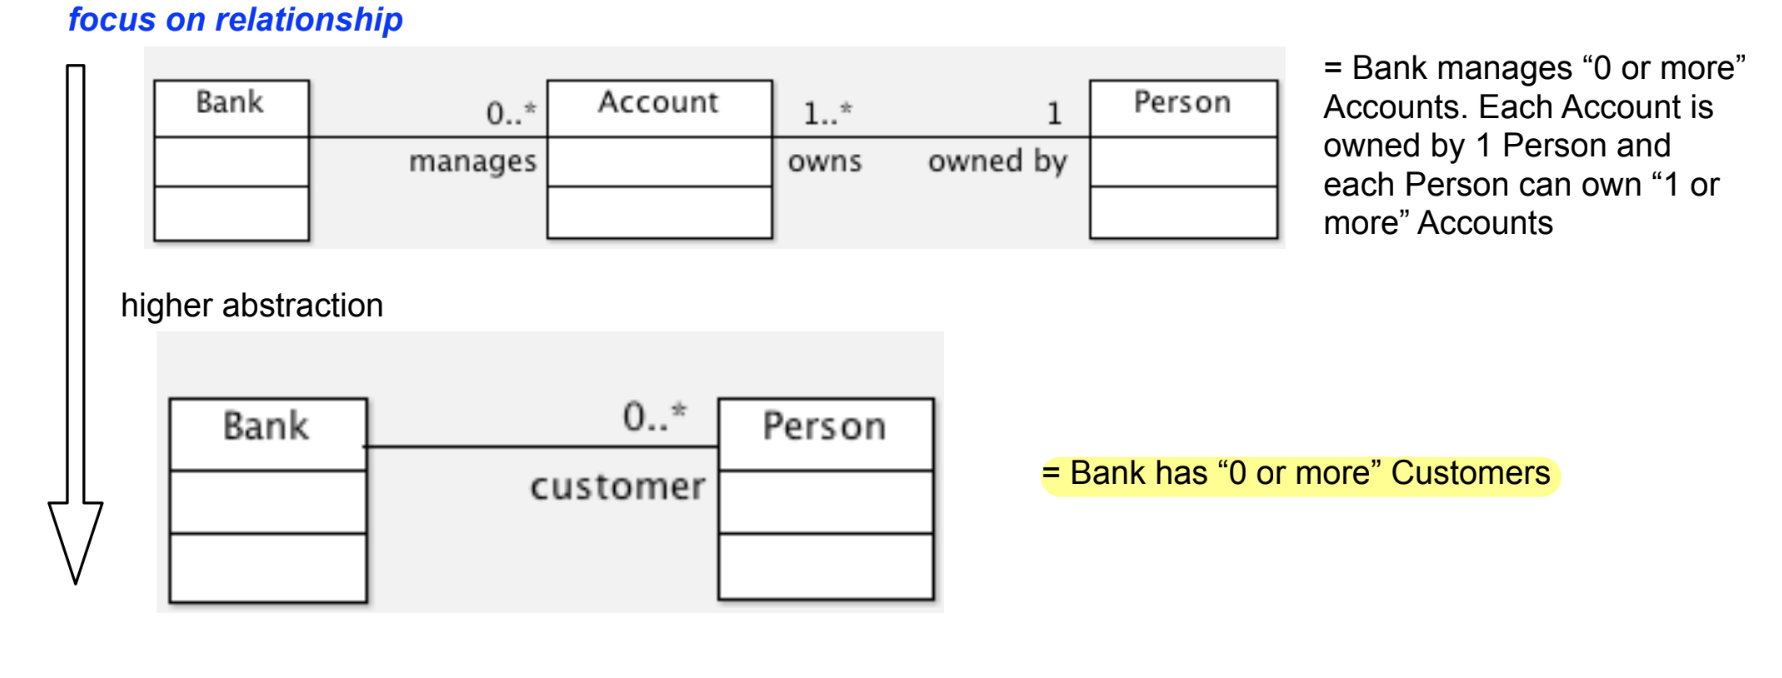
\includegraphics[width = 0.6\linewidth]{Pictures/Screenshot 2023-01-27 at 12.16.58.png}
\end{figure}
At some points, might be best to get rid of all methods and attributes to just focus on relationships.
\subsection{Association}
In class box, we represent attributes as a line of text i.e a reference to a Time Object:
\begin{figure}[H]
\centering
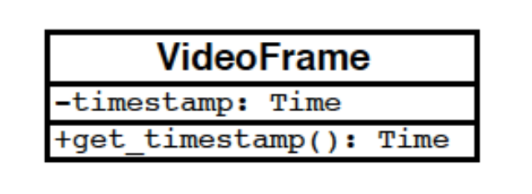
\includegraphics[width = 0.3\linewidth]{Pictures/Screenshot 2023-01-27 at 12.18.38.png}
\end{figure}
But, we can also show that using association, with a solid line with an arrow. This indicates that the class uses an attribute of that object. This is mostly used for more significant classes.
\begin{figure}[H]
\centering
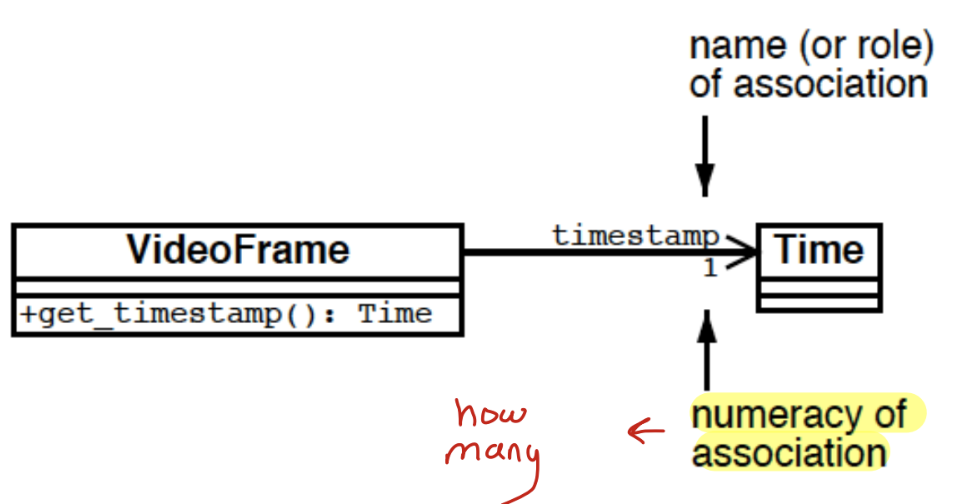
\includegraphics[width = 0.6\linewidth]{Pictures/Screenshot 2023-01-27 at 12.20.22.png}
\end{figure}
This line is:
\begin{itemize}
    \item Directional - unidirectional association
    \item Meaningful - need to name what the attribute is defined as in the class
    \item Constrained - it is stated how many Time objects a VideoFrame can be in this relationship at the same time i.e 1. This can also be a range e.g 0..1, * (infinite amount) or 1..* (at least 1)
\end{itemize}
\subsection{Navigability}
These associations can also do bidirectional navigability, as seen below.
\begin{figure}[H]
\centering
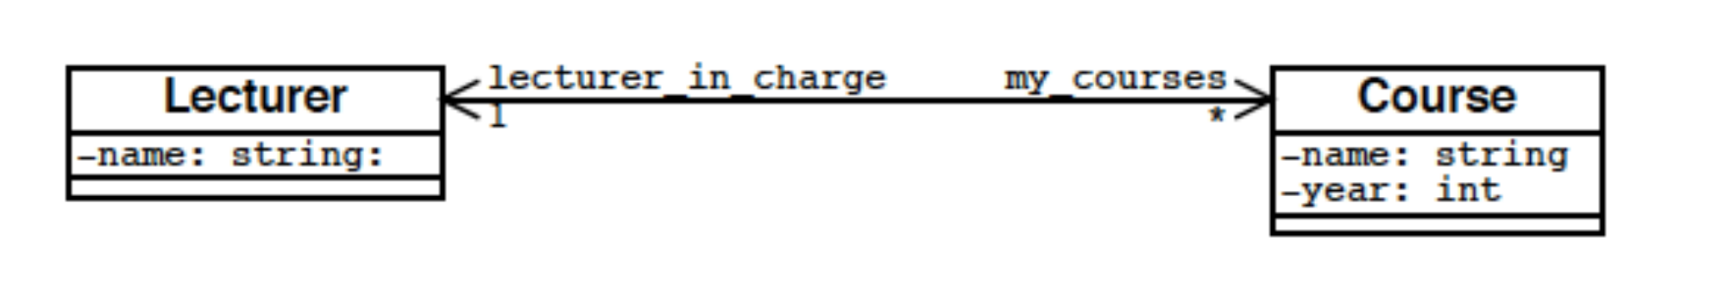
\includegraphics[width = 0.6\linewidth]{Pictures/Screenshot 2023-01-27 at 12.23.32.png}
\end{figure}
From this we can see that each Lecturer object knows about all the courses they are teaching, and * indicates that they can be in charge of any number of courses. For each Course, there is only 1 lecture in charge. \\
We might not show the directional of associations if it is not relevant to the meaning of the diagram.
\subsection{Composition - don't need to draw this in exam}
We can include a diamond when having class association. A filled diamond indicates composition
\begin{figure}[H]
\centering
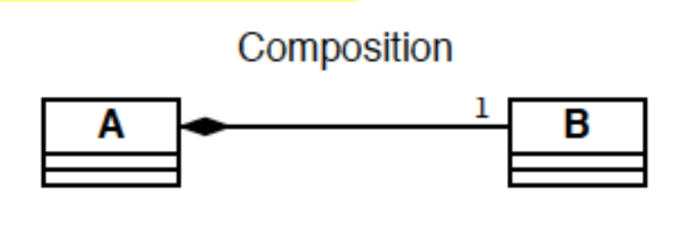
\includegraphics[width = 0.3\linewidth]{Pictures/Screenshot 2023-01-27 at 12.27.25.png}
\end{figure}
This means that if A is destroyed, then B will be destroyed too. These are good to show the strength of relationship between classes i.e exclusive ownership.
\subsection{Aggregation - don't need to draw this in exam}
An empty diamond means objects of class A contain objects of class B. But A doesn't control the lifecycle of B i.e destroying A doesn't destroy B. \\
For example, a college society has students, but closing the society won't destroy the students.
\begin{figure}[H]
\centering
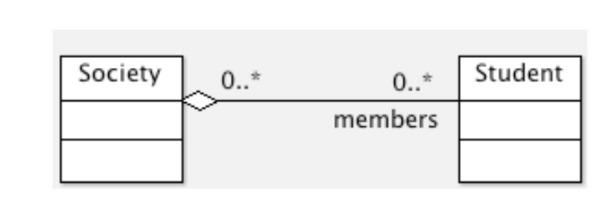
\includegraphics[width = 0.6\linewidth]{Pictures/Screenshot 2023-01-27 at 12.30.49.png}
\end{figure}
\subsection{Inheritance}
We can represent inheritance between classes as:
\begin{figure}[H]
\centering
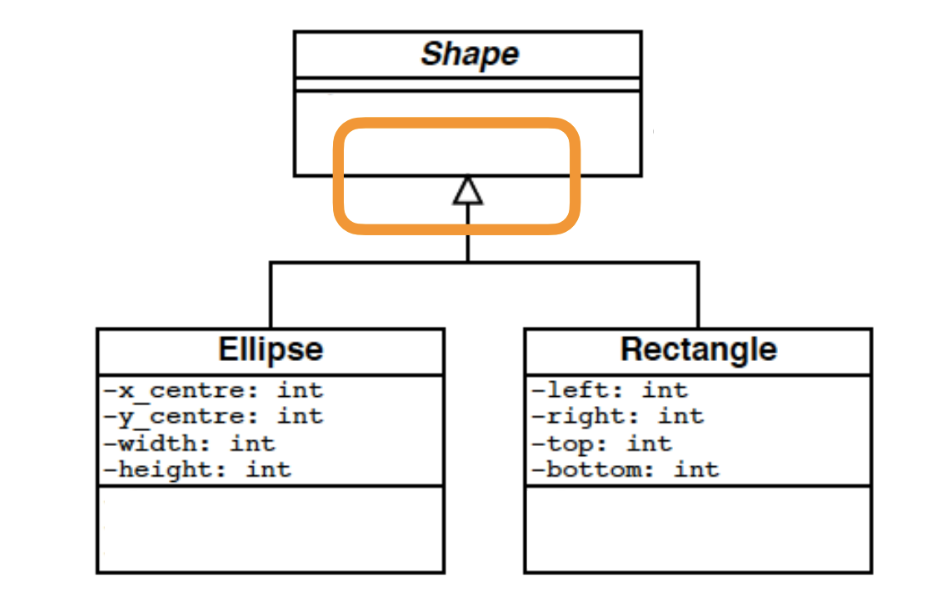
\includegraphics[width = 0.5\linewidth]{Pictures/Screenshot 2023-01-27 at 12.32.13.png}
\end{figure}
\subsection{Abstract Methods}
We can include abstract classes and methods in UML using italics. This can be hard to do in handwriting, so instead, can mark a class/method as \{abstract\}. If a class has an abstract method, then it must be declared as an abstract class.
\begin{figure}[H]
\centering
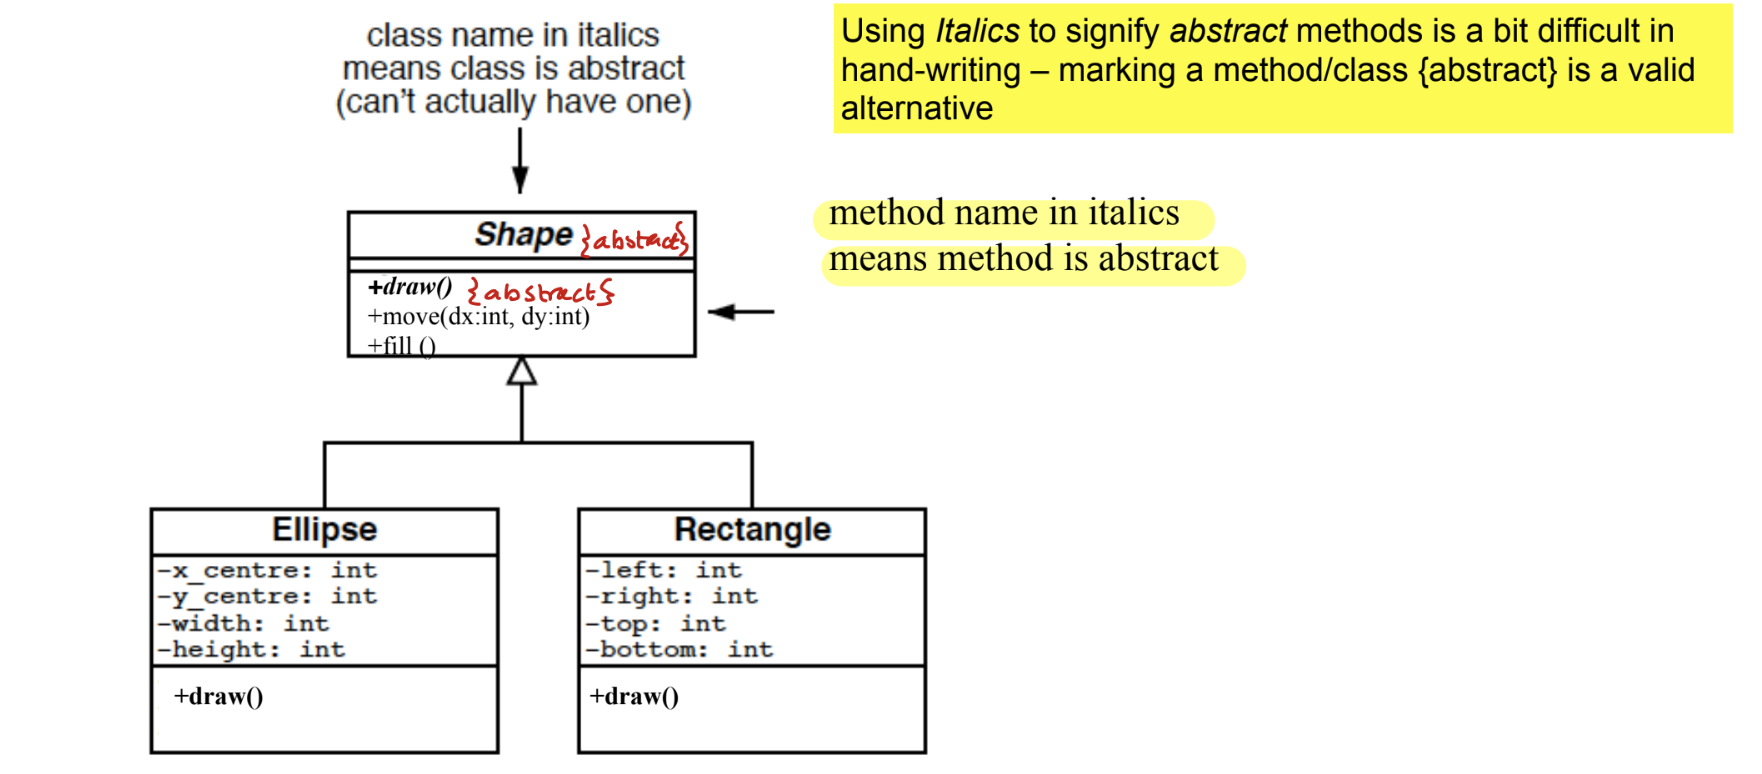
\includegraphics[width = 0.6\linewidth]{Pictures/Screenshot 2023-01-27 at 12.34.03.png}
\end{figure}
\subsection{Interfaces}
Inheritance is useful when:
\begin{itemize}
    \item Implementation inheritance - superclass implements some functionality which can be re-used by all subclasses
    \item Behaviour inheritance - class can expose a certain set of functionality
\end{itemize}
We can use interfaces for methods which might be access by different subclasses, as seen in \hyperref[interface]{Interfaces}. 
\begin{figure}[H]
\centering
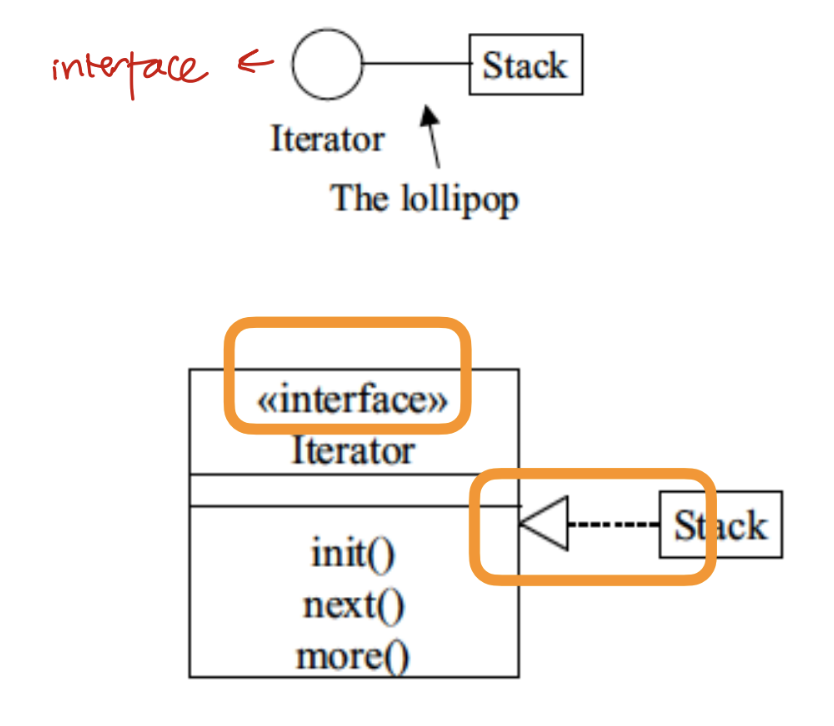
\includegraphics[width = 0.5\linewidth]{Pictures/Screenshot 2023-01-27 at 12.38.37.png}
\caption{UML Interface}
\end{figure}
It is also common to start interface names with the letter I. Interfaces are great to apply the same functionality to very different concepts, like comparing apples to oranges.
\begin{figure}[H]
\centering
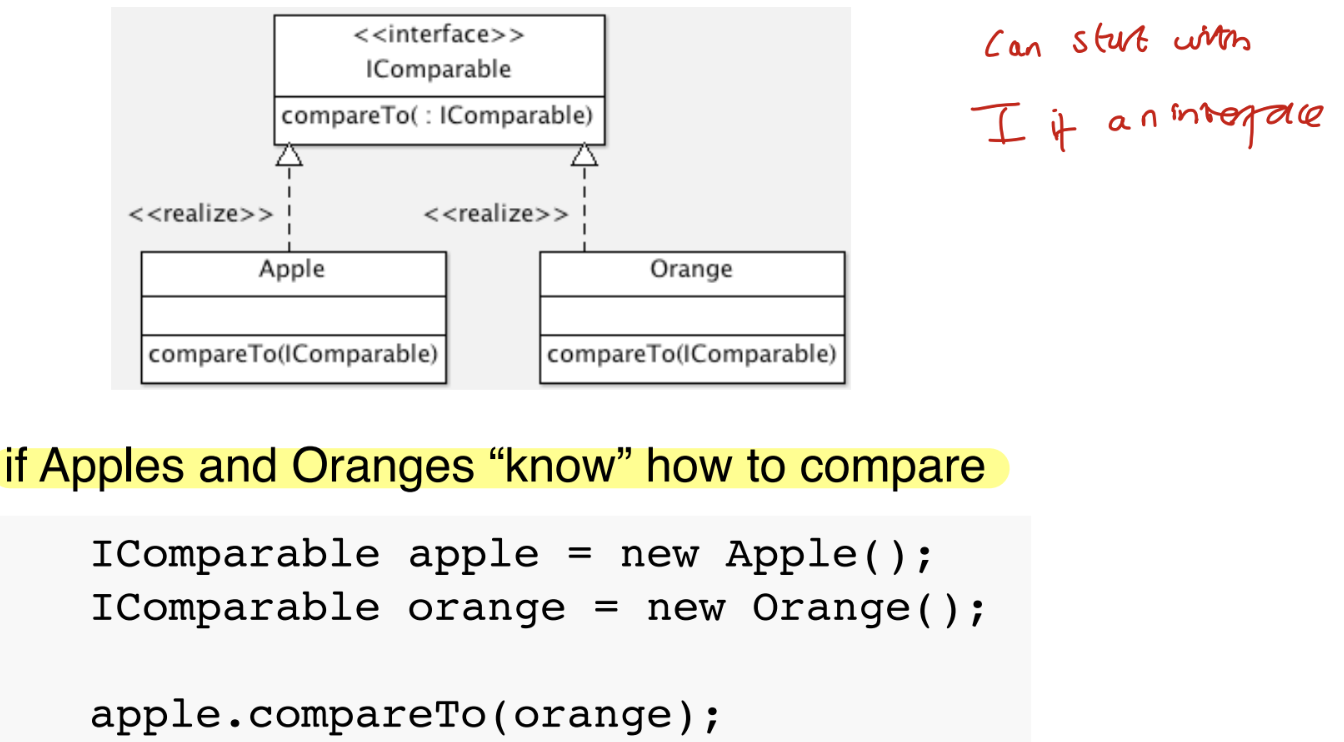
\includegraphics[width = 0.6\linewidth]{Pictures/Screenshot 2023-01-27 at 12.40.28.png}
\end{figure}
\subsection{Class Diagram Example}
\begin{figure}[H]
\centering
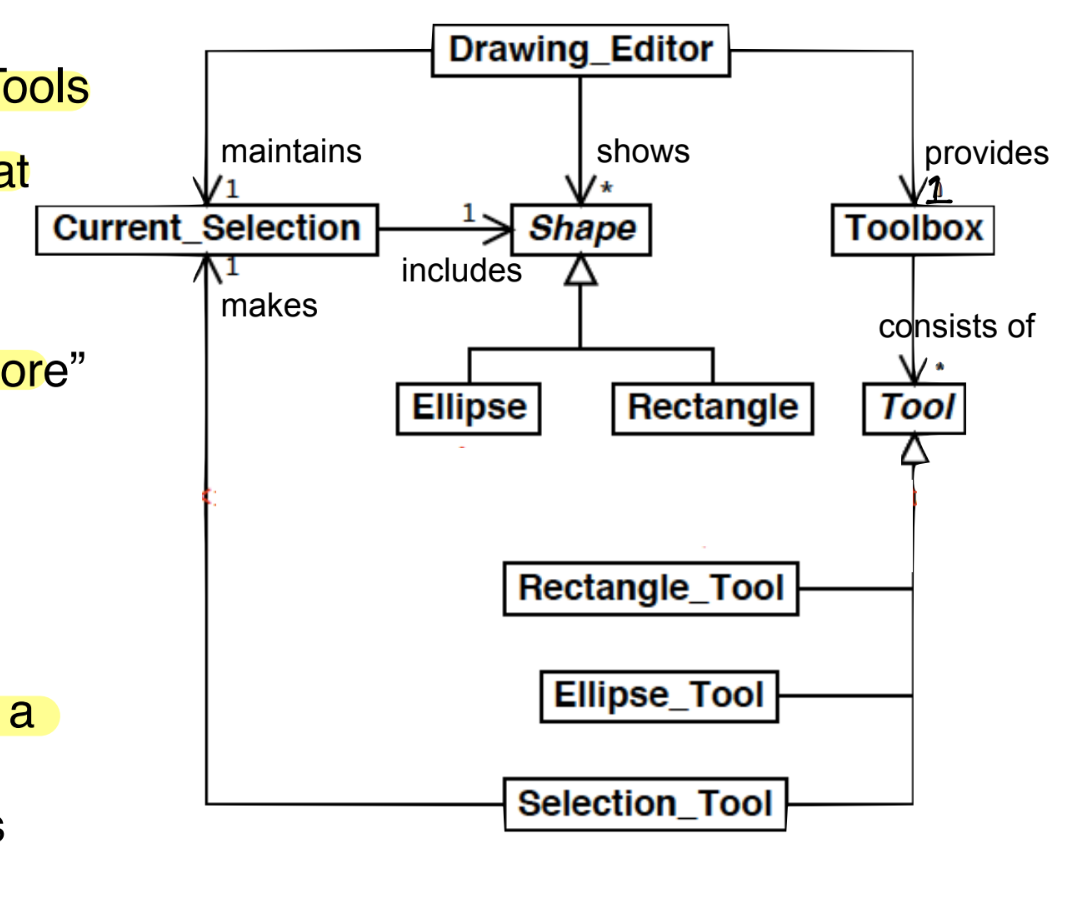
\includegraphics[width = 0.5\linewidth]{Pictures/Screenshot 2023-01-27 at 12.41.28.png}
\caption{Drawing Editor Class}
\end{figure}
Explaining this diagram:
\begin{itemize}
    \item Drawing Editor has 1 Toolbox
    \item Toolbox has any number of Tools
    \item There are 3 types of Tools: Rectangles, Ellipses and make a Selection
    \item The Drawing Editor can show any number of shapes
    \item There are 2 types of shapes: Ellipses and Rectangles
    \item Drawing Editor maintains the current Selection
    \item Only 1 shape can be selected at once
\end{itemize}
\subsection{Dynamic View}
Class Diagrams are good for capturing the relationships, but we need to use dynamic diagrams to show how objects interact with each other for a particular action. There are 2 choices:
\begin{itemize}
    \item Sequence diagrams - they present a more clear view of the timeline. They are easier to read when there are a few objects, with a lot of calls.
    \item Communication diagrams - they focus more on the nature of collaboration between the object to perform an action. They are better if there are a few method calls between many objects.
\end{itemize}
To look at both of them, we can use a drawing editor example:
\begin{figure}[H]
\centering
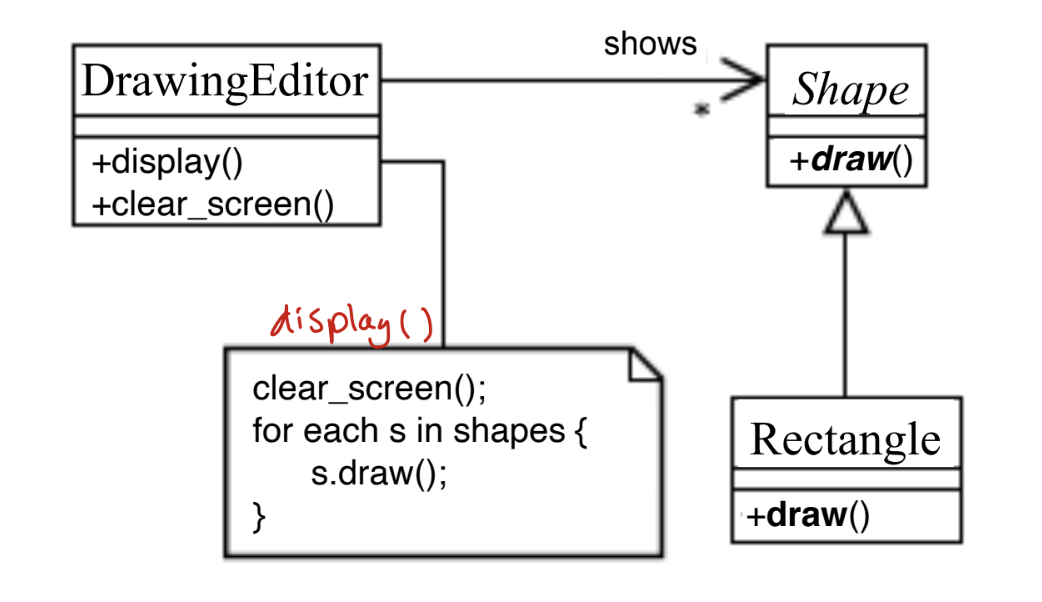
\includegraphics[width = 0.5\linewidth]{Pictures/Screenshot 2023-01-27 at 12.46.49.png}
\end{figure}
If we call the display() method, then we can look at each diagram and how it works:
\subsection{Sequence Diagram}
A Sequence diagram has a vertical axis, representing time, and white boxes to show the duration of each call.
\begin{figure}[H]
\centering
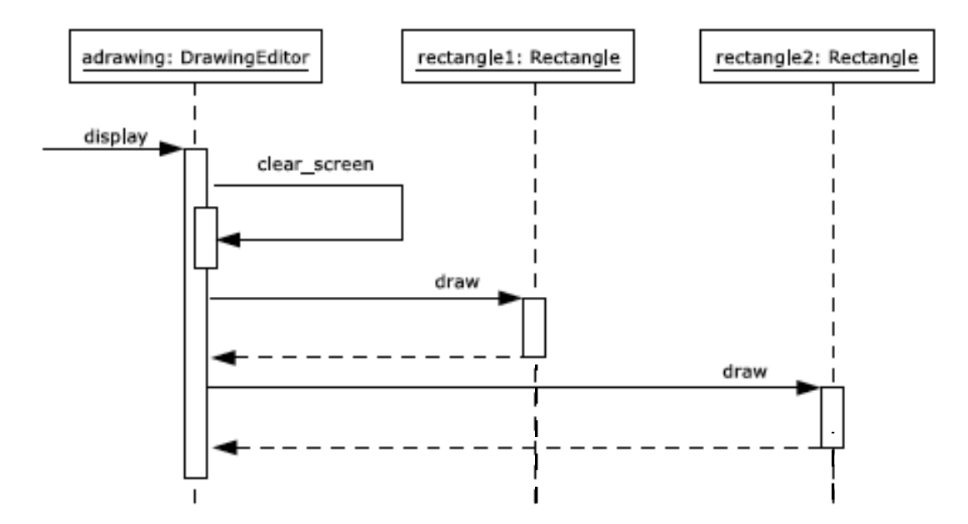
\includegraphics[width = 0.6\linewidth]{Pictures/Screenshot 2023-01-27 at 12.48.22.png}
\caption{Sequence Diagram}
\end{figure}
This works by:
\begin{itemize}
    \item display() is called in adrawing
    \item adrawing calls the clear\_screen() method on itself
    \item adrawing calls the draw() method in rectangle1, which returns
    \item adrawing calls the draw() method in rectangle2, which returns
    \item the display() method is completed
\end{itemize}
We don't always need to include the return from the draw() class (in dashed lines).
\subsection{Communication Diagram}
These show the method flow between objects, by numbering method calls:
\begin{figure}[H]
\centering
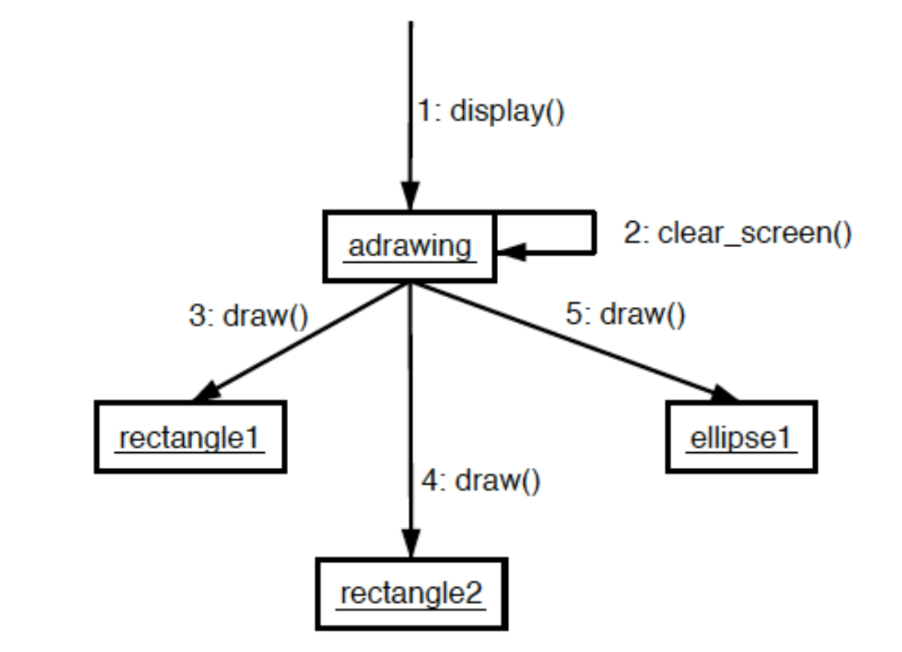
\includegraphics[width = 0.5\linewidth]{Pictures/Screenshot 2023-01-27 at 12.51.42.png}
\caption{Communication Diagram}
\end{figure}
\subsection{State Diagrams}
If the behaviour of an object depends on its state e.g in embedded software, then we can use UML State Diagrams to show it
\begin{figure}[H]
\centering
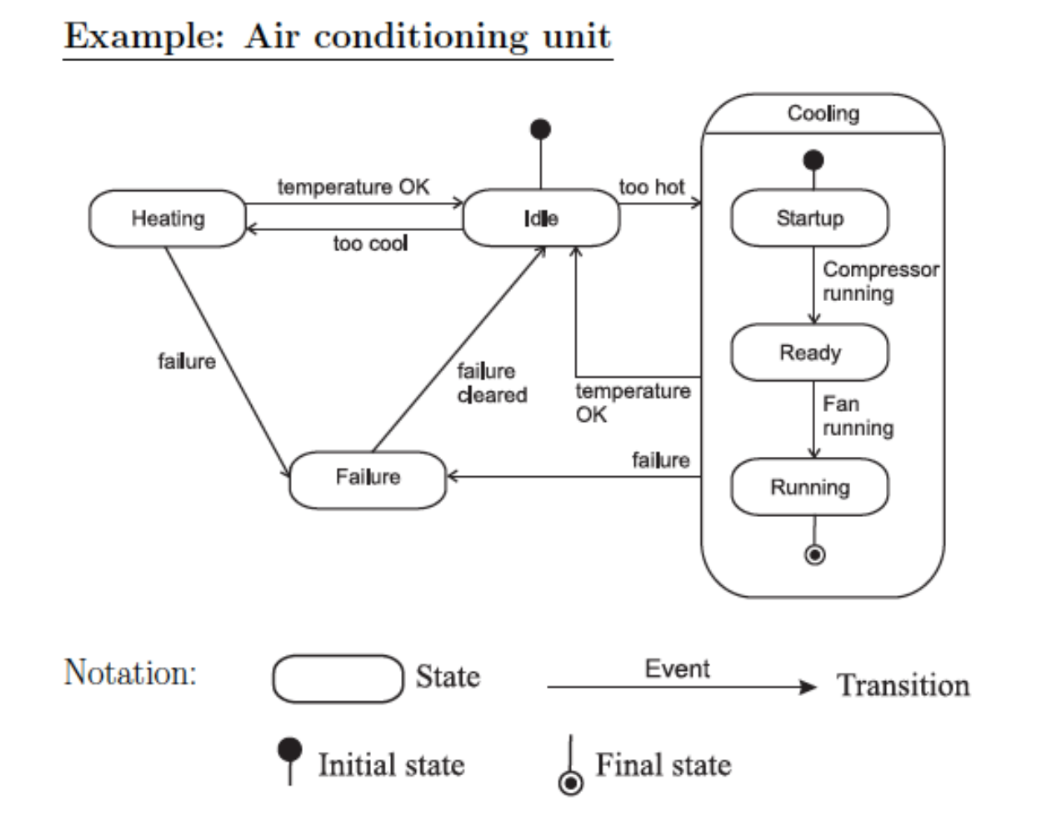
\includegraphics[width = 0.5\linewidth]{Pictures/Screenshot 2023-01-27 at 12.52.49.png}
\caption{State Diagram}
\end{figure}
\subsection{New Notation}
Project Teams can expand UML to their own needs, as long as everyone on the project can understand it, and everyone's understanding is the same
\begin{figure}[H]
\centering
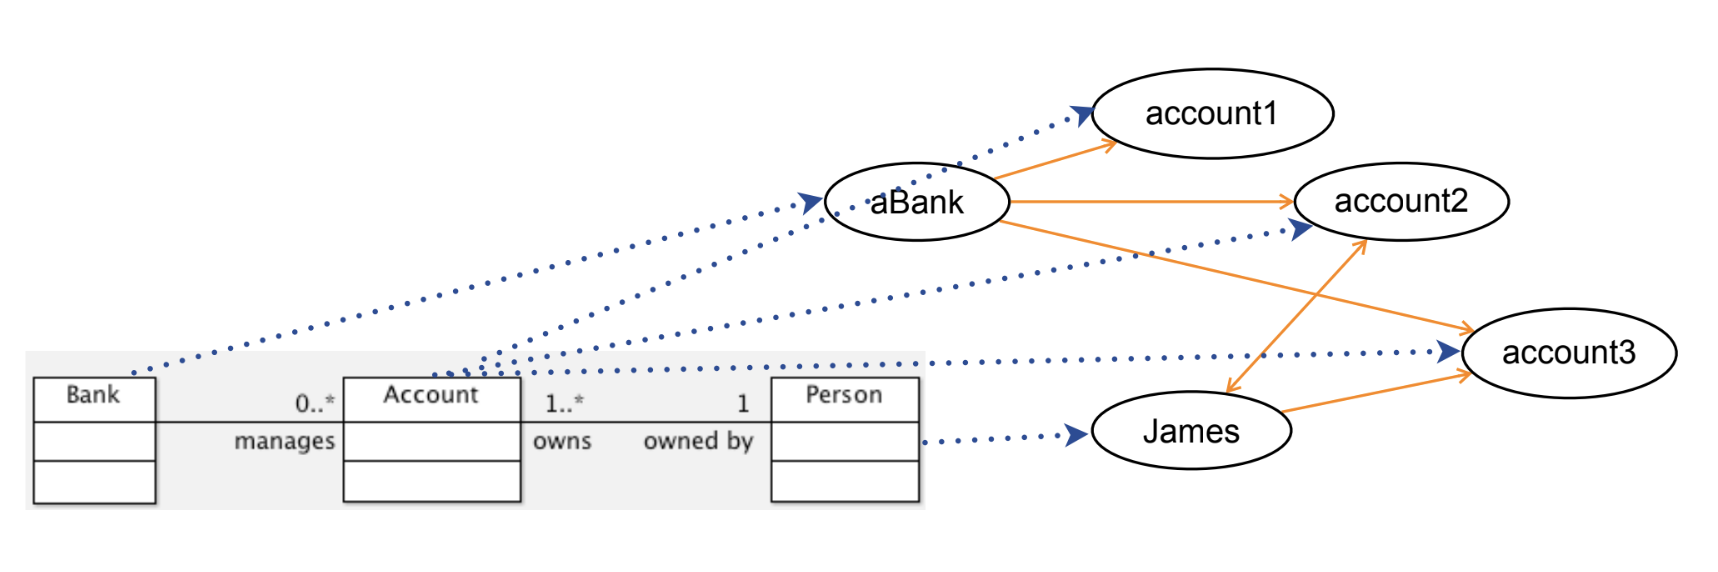
\includegraphics[width = 0.6\linewidth]{Pictures/Screenshot 2023-01-27 at 12.54.30.png}
\end{figure}
\end{document}
